\documentclass{standalone}
\usepackage{tikz}
\usetikzlibrary{patterns, positioning}
\usepackage[sfdefault]{ClearSans} %% option 'sfdefault' activates Clear Sans as the default text font
\usepackage[T1]{fontenc}

\begin{document}
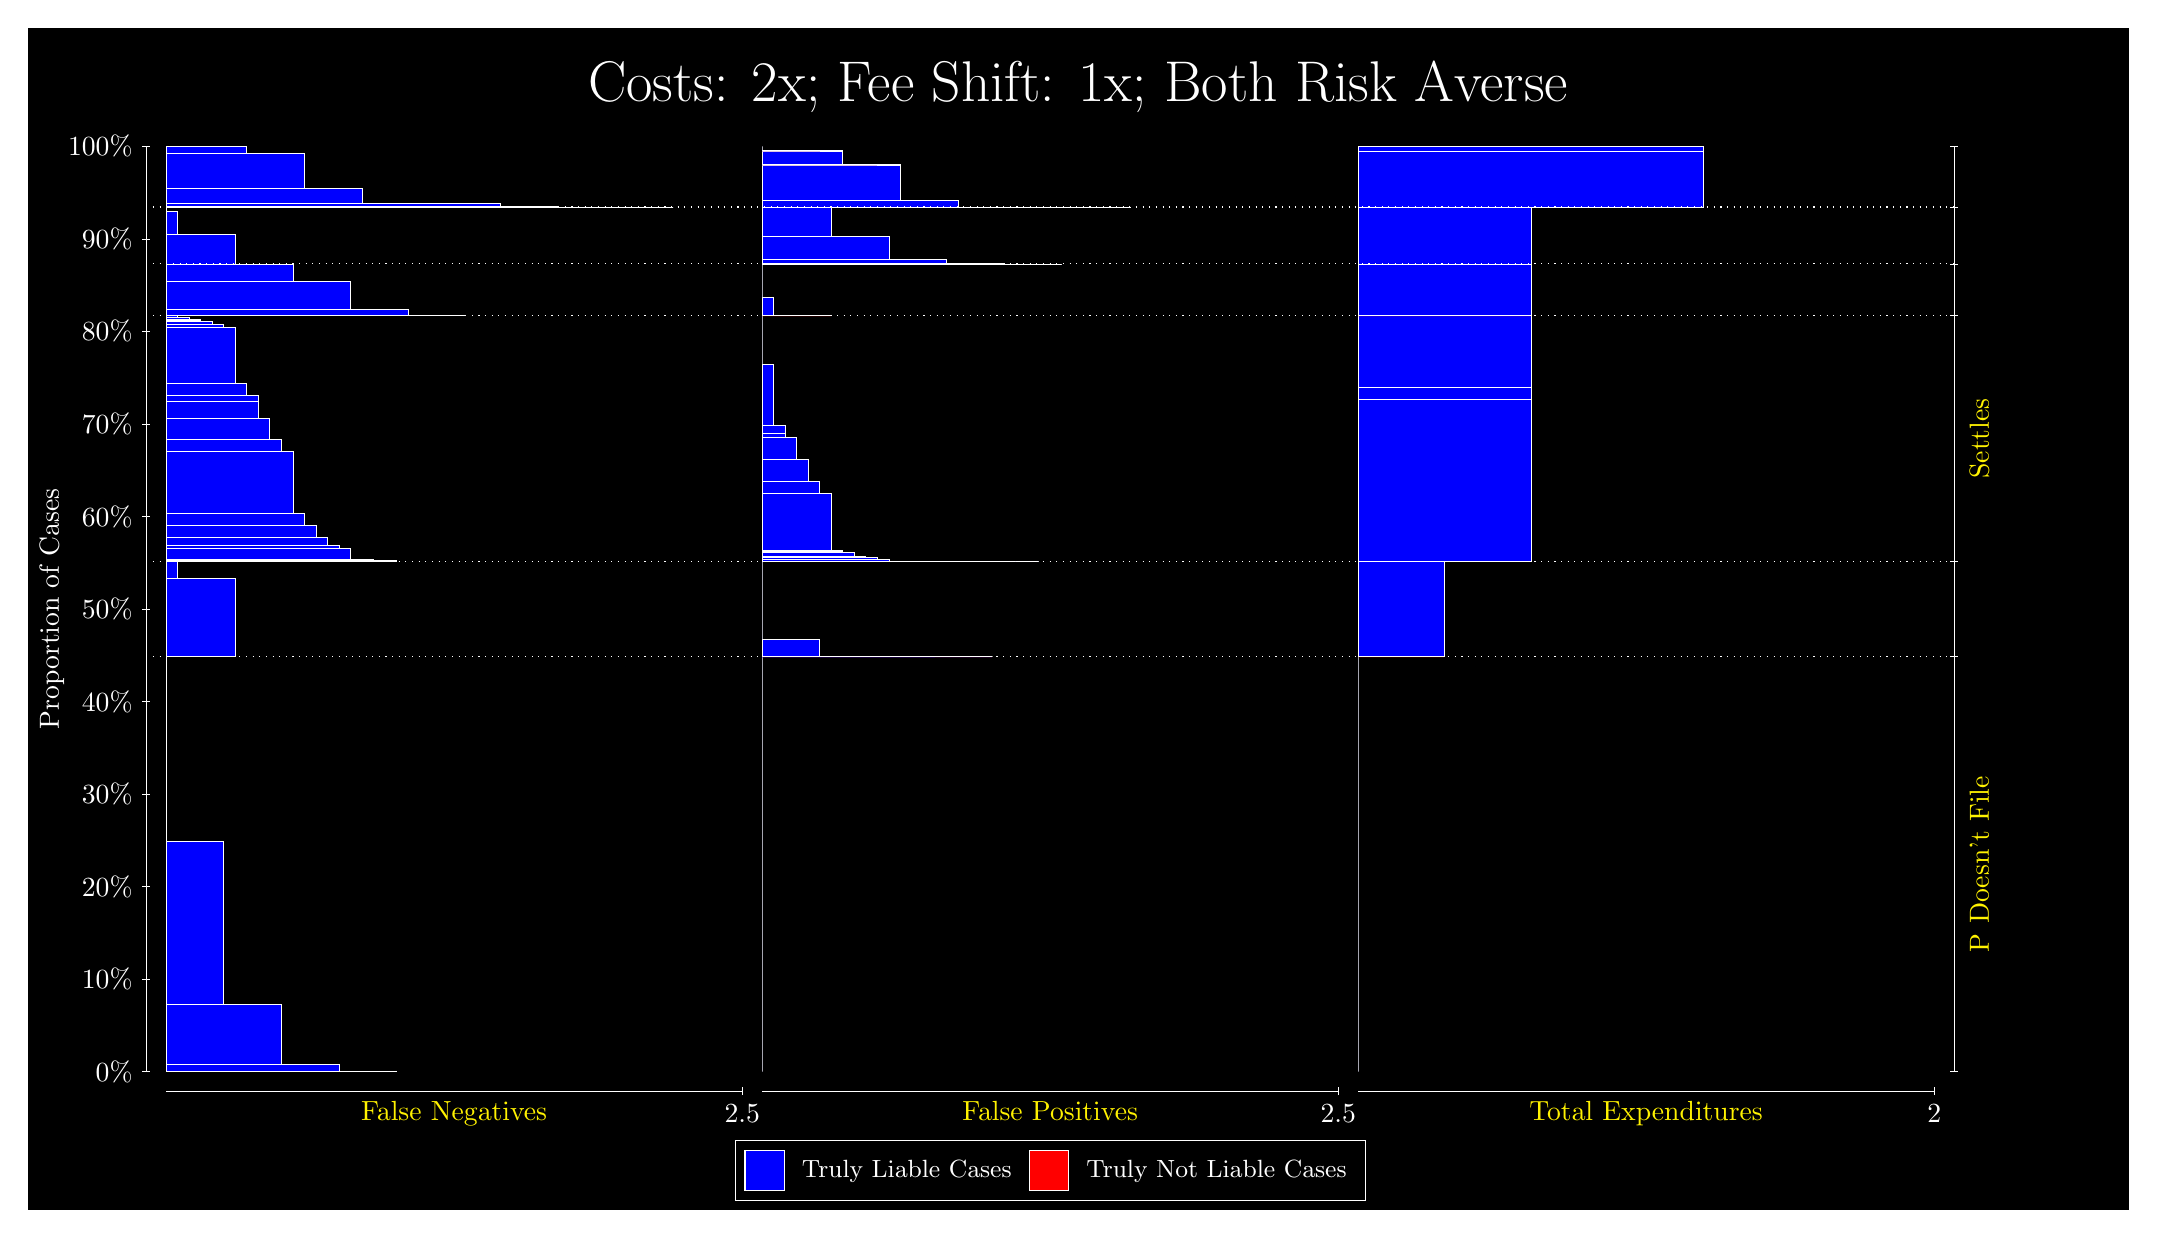
\begin{tikzpicture}
\draw[fill=black] (0,0) rectangle (26.667,15);
\draw[text=white] (0,13.5) rectangle (26.667,15) node[midway] {\huge Costs: 2x; Fee Shift: 1x; Both Risk Averse};
\draw[white, very thin] (1.5,1.75) -- (1.5,13.5);
\node[rotate=90, text=white, anchor=center] at (0.3, 7.625) {Proportion of Cases};
\draw[white, very thin] (1.45,1.75) -- (1.55,1.75);
\node[text=white, anchor=east] at (1.45, 1.75) {0\%};
\draw[white, very thin] (1.45,2.925) -- (1.55,2.925);
\node[text=white, anchor=east] at (1.45, 2.925) {10\%};
\draw[white, very thin] (1.45,4.1) -- (1.55,4.1);
\node[text=white, anchor=east] at (1.45, 4.1) {20\%};
\draw[white, very thin] (1.45,5.275) -- (1.55,5.275);
\node[text=white, anchor=east] at (1.45, 5.275) {30\%};
\draw[white, very thin] (1.45,6.45) -- (1.55,6.45);
\node[text=white, anchor=east] at (1.45, 6.45) {40\%};
\draw[white, very thin] (1.45,7.625) -- (1.55,7.625);
\node[text=white, anchor=east] at (1.45, 7.625) {50\%};
\draw[white, very thin] (1.45,8.8) -- (1.55,8.8);
\node[text=white, anchor=east] at (1.45, 8.8) {60\%};
\draw[white, very thin] (1.45,9.975) -- (1.55,9.975);
\node[text=white, anchor=east] at (1.45, 9.975) {70\%};
\draw[white, very thin] (1.45,11.15) -- (1.55,11.15);
\node[text=white, anchor=east] at (1.45, 11.15) {80\%};
\draw[white, very thin] (1.45,12.325) -- (1.55,12.325);
\node[text=white, anchor=east] at (1.45, 12.325) {90\%};
\draw[white, very thin] (1.45,13.5) -- (1.55,13.5);
\node[text=white, anchor=east] at (1.45, 13.5) {100\%};

\draw[white, very thin] (24.457,1.75) -- (24.457,13.5);
\draw[white, very thin] (24.407,1.75) -- (24.507,1.75);
\node[anchor=west] at (24.407, 1.75) {};
\draw[white, very thin] (24.407,7.0188) -- (24.507,7.0188);
\node[anchor=west] at (24.407, 7.0188) {};
\draw[white, very thin] (24.407,8.2311) -- (24.507,8.2311);
\node[anchor=west] at (24.407, 8.2311) {};
\draw[white, very thin] (24.407,11.349) -- (24.507,11.349);
\node[anchor=west] at (24.407, 11.349) {};
\draw[white, very thin] (24.407,12.008) -- (24.507,12.008);
\node[anchor=west] at (24.407, 12.008) {};
\draw[white, very thin] (24.407,12.729) -- (24.507,12.729);
\node[anchor=west] at (24.407, 12.729) {};
\draw[white, very thin] (24.407,13.5) -- (24.507,13.5);
\node[anchor=west] at (24.407, 13.5) {};

\draw[white, very thin, fill=blue] (1.75,1.75) rectangle (4.6775,1.7509);
\draw[white, very thin, fill=blue] (1.75,1.7509) rectangle (3.9457,1.8438);
\draw[white, very thin, fill=blue] (1.75,1.8438) rectangle (3.2138,2.6053);
\draw[white, very thin, fill=blue] (1.75,2.6053) rectangle (2.4819,4.6716);
\draw[white, very thin, fill=red] (1.75,4.6716) rectangle (1.75,4.6716);
\draw[white, very thin, fill=blue] (1.75,4.6716) rectangle (1.75,7.0188);
\draw[white, very thin, fill=blue] (1.75,7.0188) rectangle (2.6283,8.0107);
\draw[white, very thin, fill=blue] (1.75,8.0107) rectangle (1.8964,8.2249);
\draw[white, very thin, fill=red] (1.75,8.2249) rectangle (1.75,8.2249);
\draw[white, very thin, fill=blue] (1.75,8.2249) rectangle (1.75,8.2311);
\draw[white, very thin, fill=blue] (1.75,8.2311) rectangle (4.6775,8.2367);
\draw[white, very thin, fill=blue] (1.75,8.2367) rectangle (4.3848,8.2499);
\draw[white, very thin, fill=blue] (1.75,8.2499) rectangle (4.092,8.3926);
\draw[white, very thin, fill=blue] (1.75,8.3926) rectangle (3.9457,8.4335);
\draw[white, very thin, fill=blue] (1.75,8.4335) rectangle (3.7993,8.541);
\draw[white, very thin, fill=blue] (1.75,8.541) rectangle (3.6529,8.6898);
\draw[white, very thin, fill=blue] (1.75,8.6898) rectangle (3.5065,8.8436);
\draw[white, very thin, fill=blue] (1.75,8.8436) rectangle (3.3602,9.6269);
\draw[white, very thin, fill=blue] (1.75,9.6269) rectangle (3.2138,9.7732);
\draw[white, very thin, fill=blue] (1.75,9.7732) rectangle (3.0674,10.05);
\draw[white, very thin, fill=blue] (1.75,10.05) rectangle (2.921,10.268);
\draw[white, very thin, fill=blue] (1.75,10.268) rectangle (2.921,10.339);
\draw[white, very thin, fill=blue] (1.75,10.339) rectangle (2.7746,10.49);
\draw[white, very thin, fill=blue] (1.75,10.49) rectangle (2.6283,11.204);
\draw[white, very thin, fill=blue] (1.75,11.204) rectangle (2.4819,11.238);
\draw[white, very thin, fill=blue] (1.75,11.238) rectangle (2.3355,11.282);
\draw[white, very thin, fill=blue] (1.75,11.282) rectangle (2.1891,11.29);
\draw[white, very thin, fill=blue] (1.75,11.29) rectangle (2.1891,11.305);
\draw[white, very thin, fill=blue] (1.75,11.305) rectangle (2.0428,11.324);
\draw[white, very thin, fill=blue] (1.75,11.324) rectangle (1.8964,11.349);
\draw[white, very thin, fill=red] (1.75,11.349) rectangle (1.75,11.349);
\draw[white, very thin, fill=blue] (1.75,11.349) rectangle (1.75,11.349);
\draw[white, very thin, fill=blue] (1.75,11.349) rectangle (5.5558,11.356);
\draw[white, very thin, fill=blue] (1.75,11.356) rectangle (4.8239,11.427);
\draw[white, very thin, fill=blue] (1.75,11.427) rectangle (4.092,11.78);
\draw[white, very thin, fill=blue] (1.75,11.78) rectangle (3.3602,12.005);
\draw[white, very thin, fill=blue] (1.75,12.005) rectangle (2.6283,12.008);
\draw[white, very thin, fill=red] (1.75,12.008) rectangle (1.75,12.008);
\draw[white, very thin, fill=blue] (1.75,12.008) rectangle (2.6283,12.385);
\draw[white, very thin, fill=blue] (1.75,12.385) rectangle (1.8964,12.676);
\draw[white, very thin, fill=red] (1.75,12.676) rectangle (1.75,12.676);
\draw[white, very thin, fill=blue] (1.75,12.676) rectangle (1.75,12.729);
\draw[white, very thin, fill=blue] (1.75,12.729) rectangle (8.1906,12.729);
\draw[white, very thin, fill=blue] (1.75,12.729) rectangle (7.4587,12.73);
\draw[white, very thin, fill=blue] (1.75,12.73) rectangle (6.7268,12.743);
\draw[white, very thin, fill=blue] (1.75,12.743) rectangle (5.9949,12.774);
\draw[white, very thin, fill=blue] (1.75,12.774) rectangle (5.7022,12.774);
\draw[white, very thin, fill=blue] (1.75,12.774) rectangle (5.2631,12.776);
\draw[white, very thin, fill=blue] (1.75,12.776) rectangle (4.9703,12.783);
\draw[white, very thin, fill=blue] (1.75,12.783) rectangle (4.5312,12.783);
\draw[white, very thin, fill=blue] (1.75,12.783) rectangle (4.2384,12.963);
\draw[white, very thin, fill=blue] (1.75,12.963) rectangle (3.7993,12.963);
\draw[white, very thin, fill=blue] (1.75,12.963) rectangle (3.5065,13.417);
\draw[white, very thin, fill=blue] (1.75,13.417) rectangle (2.7746,13.498);
\draw[white, very thin, fill=blue] (1.75,13.498) rectangle (2.0428,13.5);
\draw[white, very thin, fill=red] (1.75,13.5) rectangle (1.75,13.5);
\draw[white, very thin, fill=blue] (1.75,13.5) rectangle (1.75,13.5);
\draw[white, very thin, fill=red] (9.3189,1.75) rectangle (9.3189,1.75);
\draw[white, very thin, fill=blue] (9.3189,1.75) rectangle (9.3189,7.0188);
\draw[white, very thin, fill=red] (9.3189,7.0188) rectangle (12.246,7.0188);
\draw[white, very thin, fill=blue] (9.3189,7.0188) rectangle (12.246,7.0188);
\draw[white, very thin, fill=blue] (9.3189,7.0188) rectangle (11.515,7.0188);
\draw[white, very thin, fill=blue] (9.3189,7.0188) rectangle (10.783,7.0249);
\draw[white, very thin, fill=blue] (9.3189,7.0249) rectangle (10.051,7.2391);
\draw[white, very thin, fill=blue] (9.3189,7.2391) rectangle (9.3189,8.2311);
\draw[white, very thin, fill=red] (9.3189,8.2311) rectangle (12.832,8.2311);
\draw[white, very thin, fill=blue] (9.3189,8.2311) rectangle (12.832,8.2311);
\draw[white, very thin, fill=red] (9.3189,8.2311) rectangle (12.539,8.2311);
\draw[white, very thin, fill=blue] (9.3189,8.2311) rectangle (12.539,8.2311);
\draw[white, very thin, fill=red] (9.3189,8.2311) rectangle (12.246,8.2311);
\draw[white, very thin, fill=blue] (9.3189,8.2311) rectangle (12.246,8.2311);
\draw[white, very thin, fill=blue] (9.3189,8.2311) rectangle (12.1,8.2311);
\draw[white, very thin, fill=red] (9.3189,8.2311) rectangle (11.954,8.2311);
\draw[white, very thin, fill=blue] (9.3189,8.2311) rectangle (11.954,8.2311);
\draw[white, very thin, fill=blue] (9.3189,8.2311) rectangle (11.807,8.2311);
\draw[white, very thin, fill=red] (9.3189,8.2311) rectangle (11.661,8.2311);
\draw[white, very thin, fill=blue] (9.3189,8.2311) rectangle (11.661,8.2311);
\draw[white, very thin, fill=blue] (9.3189,8.2311) rectangle (11.515,8.2311);
\draw[white, very thin, fill=red] (9.3189,8.2311) rectangle (11.368,8.2311);
\draw[white, very thin, fill=blue] (9.3189,8.2311) rectangle (11.368,8.2311);
\draw[white, very thin, fill=blue] (9.3189,8.2311) rectangle (11.222,8.2312);
\draw[white, very thin, fill=blue] (9.3189,8.2312) rectangle (11.075,8.2313);
\draw[white, very thin, fill=red] (9.3189,8.2313) rectangle (11.075,8.2313);
\draw[white, very thin, fill=blue] (9.3189,8.2313) rectangle (11.075,8.2314);
\draw[white, very thin, fill=blue] (9.3189,8.2314) rectangle (10.929,8.2562);
\draw[white, very thin, fill=blue] (9.3189,8.2562) rectangle (10.783,8.2752);
\draw[white, very thin, fill=blue] (9.3189,8.2752) rectangle (10.636,8.2982);
\draw[white, very thin, fill=blue] (9.3189,8.2982) rectangle (10.49,8.342);
\draw[white, very thin, fill=blue] (9.3189,8.342) rectangle (10.344,8.3541);
\draw[white, very thin, fill=blue] (9.3189,8.3541) rectangle (10.344,8.3756);
\draw[white, very thin, fill=blue] (9.3189,8.3756) rectangle (10.197,9.0901);
\draw[white, very thin, fill=blue] (9.3189,9.0901) rectangle (10.051,9.2405);
\draw[white, very thin, fill=blue] (9.3189,9.2405) rectangle (9.9044,9.5299);
\draw[white, very thin, fill=blue] (9.3189,9.5299) rectangle (9.758,9.8067);
\draw[white, very thin, fill=blue] (9.3189,9.8067) rectangle (9.6116,9.8601);
\draw[white, very thin, fill=blue] (9.3189,9.8601) rectangle (9.6116,9.953);
\draw[white, very thin, fill=blue] (9.3189,9.953) rectangle (9.4652,10.736);
\draw[white, very thin, fill=blue] (9.3189,10.736) rectangle (9.3189,11.349);
\draw[white, very thin, fill=red] (9.3189,11.349) rectangle (10.197,11.349);
\draw[white, very thin, fill=blue] (9.3189,11.349) rectangle (10.197,11.352);
\draw[white, very thin, fill=blue] (9.3189,11.352) rectangle (9.4652,11.577);
\draw[white, very thin, fill=blue] (9.3189,11.577) rectangle (9.3189,12.008);
\draw[white, very thin, fill=red] (9.3189,12.008) rectangle (13.125,12.008);
\draw[white, very thin, fill=blue] (9.3189,12.008) rectangle (13.125,12.008);
\draw[white, very thin, fill=blue] (9.3189,12.008) rectangle (12.393,12.009);
\draw[white, very thin, fill=blue] (9.3189,12.009) rectangle (11.661,12.061);
\draw[white, very thin, fill=blue] (9.3189,12.061) rectangle (10.929,12.353);
\draw[white, very thin, fill=blue] (9.3189,12.353) rectangle (10.197,12.729);
\draw[white, very thin, fill=red] (9.3189,12.729) rectangle (14.003,12.729);
\draw[white, very thin, fill=blue] (9.3189,12.729) rectangle (14.003,12.729);
\draw[white, very thin, fill=red] (9.3189,12.729) rectangle (13.271,12.729);
\draw[white, very thin, fill=blue] (9.3189,12.729) rectangle (13.271,12.729);
\draw[white, very thin, fill=red] (9.3189,12.729) rectangle (12.539,12.729);
\draw[white, very thin, fill=blue] (9.3189,12.729) rectangle (12.539,12.731);
\draw[white, very thin, fill=blue] (9.3189,12.731) rectangle (11.807,12.812);
\draw[white, very thin, fill=red] (9.3189,12.812) rectangle (11.807,12.812);
\draw[white, very thin, fill=blue] (9.3189,12.812) rectangle (11.807,12.812);
\draw[white, very thin, fill=blue] (9.3189,12.812) rectangle (11.075,13.265);
\draw[white, very thin, fill=blue] (9.3189,13.265) rectangle (11.075,13.266);
\draw[white, very thin, fill=red] (9.3189,13.266) rectangle (10.783,13.266);
\draw[white, very thin, fill=blue] (9.3189,13.266) rectangle (10.783,13.266);
\draw[white, very thin, fill=blue] (9.3189,13.266) rectangle (10.344,13.438);
\draw[white, very thin, fill=blue] (9.3189,13.438) rectangle (10.344,13.446);
\draw[white, very thin, fill=red] (9.3189,13.446) rectangle (10.051,13.446);
\draw[white, very thin, fill=blue] (9.3189,13.446) rectangle (10.051,13.446);
\draw[white, very thin, fill=blue] (9.3189,13.446) rectangle (9.6116,13.452);
\draw[white, very thin, fill=blue] (9.3189,13.452) rectangle (9.6116,13.453);
\draw[white, very thin, fill=red] (9.3189,13.453) rectangle (9.3189,13.453);
\draw[white, very thin, fill=blue] (9.3189,13.453) rectangle (9.3189,13.5);
\draw[white, very thin, fill=red] (16.888,1.75) rectangle (16.888,1.75);
\draw[white, very thin, fill=blue] (16.888,1.75) rectangle (16.888,7.0188);
\draw[white, very thin, fill=red] (16.888,7.0188) rectangle (17.986,7.0188);
\draw[white, very thin, fill=blue] (16.888,7.0188) rectangle (17.986,8.2311);
\draw[white, very thin, fill=red] (16.888,8.2311) rectangle (19.083,8.2311);
\draw[white, very thin, fill=blue] (16.888,8.2311) rectangle (19.083,10.285);
\draw[white, very thin, fill=red] (16.888,10.285) rectangle (19.083,10.285);
\draw[white, very thin, fill=blue] (16.888,10.285) rectangle (19.083,10.446);
\draw[white, very thin, fill=red] (16.888,10.446) rectangle (19.083,10.446);
\draw[white, very thin, fill=blue] (16.888,10.446) rectangle (19.083,11.349);
\draw[white, very thin, fill=red] (16.888,11.349) rectangle (19.083,11.349);
\draw[white, very thin, fill=blue] (16.888,11.349) rectangle (19.083,12.008);
\draw[white, very thin, fill=red] (16.888,12.008) rectangle (19.083,12.008);
\draw[white, very thin, fill=blue] (16.888,12.008) rectangle (19.083,12.729);
\draw[white, very thin, fill=red] (16.888,12.729) rectangle (21.279,12.729);
\draw[white, very thin, fill=blue] (16.888,12.729) rectangle (21.279,13.443);
\draw[white, very thin, fill=red] (16.888,13.443) rectangle (21.279,13.443);
\draw[white, very thin, fill=blue] (16.888,13.443) rectangle (21.279,13.5);
\draw[white, dotted] (1.5,7.0188) -- (24.457,7.0188);
\draw[white, dotted] (1.5,8.2311) -- (24.457,8.2311);
\draw[white, dotted] (1.5,11.349) -- (24.457,11.349);
\draw[white, dotted] (1.5,12.008) -- (24.457,12.008);
\draw[white, dotted] (1.5,12.729) -- (24.457,12.729);
\draw[white, very thin] (1.75,1.5) -- (9.0689,1.5);
\node[text=yellow, anchor=north] at (5.4094, 1.5) {False Negatives};
\draw[white, very thin] (9.0689,1.45) -- (9.0689,1.55);
\node[text=white, anchor=north] at (9.0689, 1.45) {2.5};

\draw[white, very thin] (9.3189,1.5) -- (16.638,1.5);
\node[text=yellow, anchor=north] at (12.978, 1.5) {False Positives};
\draw[white, very thin] (16.638,1.45) -- (16.638,1.55);
\node[text=white, anchor=north] at (16.638, 1.45) {2.5};

\draw[white, very thin] (16.888,1.5) -- (24.207,1.5);
\node[text=yellow, anchor=north] at (20.547, 1.5) {Total Expenditures};
\draw[white, very thin] (24.207,1.45) -- (24.207,1.55);
\node[text=white, anchor=north] at (24.207, 1.45) {2};

\node[text=yellow, centered, rotate=90] at (24.777, 4.3844) {P Doesn't File};

\node[text=yellow, centered, rotate=90] at (24.777, 9.79) {Settles};




\draw (12.978300999999998,1.5) node[draw=none] (baseCoordinate) {};
\begin{scope}[align=center]
        \matrix[scale=0.5, draw=white, below=0.5cm of baseCoordinate, nodes={draw}, column sep=0.1cm]{
            \node[rectangle, draw, minimum width=0.5cm, minimum height=0.5cm, fill=blue] {}; &
            \node[draw=none, font=\small, text=white] (B) {Truly Liable Cases}; &
            \node[rectangle, draw, minimum width=0.5cm, minimum height=0.5cm, fill=red] {}; &
            \node[draw=none, font=\small, text=white] (B) {Truly Not Liable Cases}; \\
            };
\end{scope}

\end{tikzpicture}
\end{document}